\documentclass[12pt,letterpaper]{article}
\usepackage[utf8]{inputenc}
\usepackage[spanish]{babel}
\usepackage{amsmath}
\usepackage{color}
\usepackage{subcaption}
\usepackage{amsfonts}
\usepackage{hyperref}
 \hypersetup{
     colorlinks=true,
     linkcolor=blue,
     filecolor=blue,
     citecolor = blue,      
     urlcolor=cyan,
     }
\usepackage{amssymb}
\usepackage{listings}
\usepackage{graphicx}
\usepackage[left=2cm,right=2cm,top=2cm,bottom=2cm]{geometry}
\setlength{\parskip}{3mm}

\title{\textsc{Práctica 2: Autómata celular}}
\author{\textsc{Fabiola Vázquez}}

\setlength{\parindent}{0cm}
\renewcommand{\lstlistingname}{Código}
\begin{document}
\maketitle

\hrule
\section{Introducción}
El juego de la vida \cite{gamelife} consiste en lo siguiente, se plantea una matriz cuadrada con unos y ceros, donde los unos representan las celdas vivas y los ceros las celdas muertas. En cada etapa del juego se analiza que la celda tenga exactamente tres vecinos vivos, si cumple la condición, vive, en caso contrario, muere. 


\section{Experimento}
Se realiza el experimento \cite{elisap2} considerando una malla de 20 por 20 y variando las probabilidades de que la celda esté viva, comenzando en 0.05 y llegando a 0.95 en incrementos de 0.05. Se hacen 50 repeticiones para cada probabilidad. Debido a que en las primeras iteraciones todas las celdas quedarán muertas, no estudiamos los casos en que la probabilidad de vivencia es cero o uno. Luego, se procede a analizar el mayor colapso poblacional entre iteraciones subsecuentes, y el mayor tiempo continuo de vida en una celda.
Dicho experimento se realiza con el software Python versión 3.7.9 \cite{python} en un cuaderno de Jupyter \cite{jupyter}.

\subsection{El mayor colapso poblacional entre iteraciones subsecuentes}
Se procede de la siguiente manera. En cada iteración se calcula la cantidad de celdas vivas. Al considerar las diferencias entre dichas cantidades, se obtiene la cantidad de celdas que murieron entre las iteraciones. Para obtener el mayor colapso poblacional,  tomamos el máximo de éstas diferencias. Los datos se almacenan en un \texttt{data frame}, que se observa parcialmente en el cuadro \ref{mcdatos}.

En la figura \ref{colapso} se tiene los gráficos de caja de cada una de las probabilidades de vivencia. En dicha figura se observa que, cuando la probabilidad de que la celda esté viva es menor que 0.5, el promedio del mayor colapso es creciente. Por el contrario, para probabilidades mayores que 0.5, el promedio disminuye.
\begin{table}
\centering
\caption{Fragmento de los datos recopilados}
\begin{tabular}{rrrrrrrr}
\hline 
Probabilidad & 1 & 2 & 3 & ... & 48 & 49 & 50 \\ 
\hline 
0.05 & 2 & 1 & 3 & ... & 1 & 1 & 2 \\ 
0.10 & 10 & 4 & 6 & ... & 16 & 12 & 9 \\ 
$\vdots$ & $\vdots$ & $\vdots$ & $\vdots$ & $\vdots$ & $\vdots$ & $\vdots$ & $\vdots$ \\ 
0.90 & 11 & 7 & 4 & ... & 8 & 5 & 7 \\ 
 0.95 & 6 & 4 & 6 & ... & 3 & 7 & 4 \\  
 \hline
\end{tabular} 
\label{mcdatos}
\end{table}



\begin{figure}
\centering
 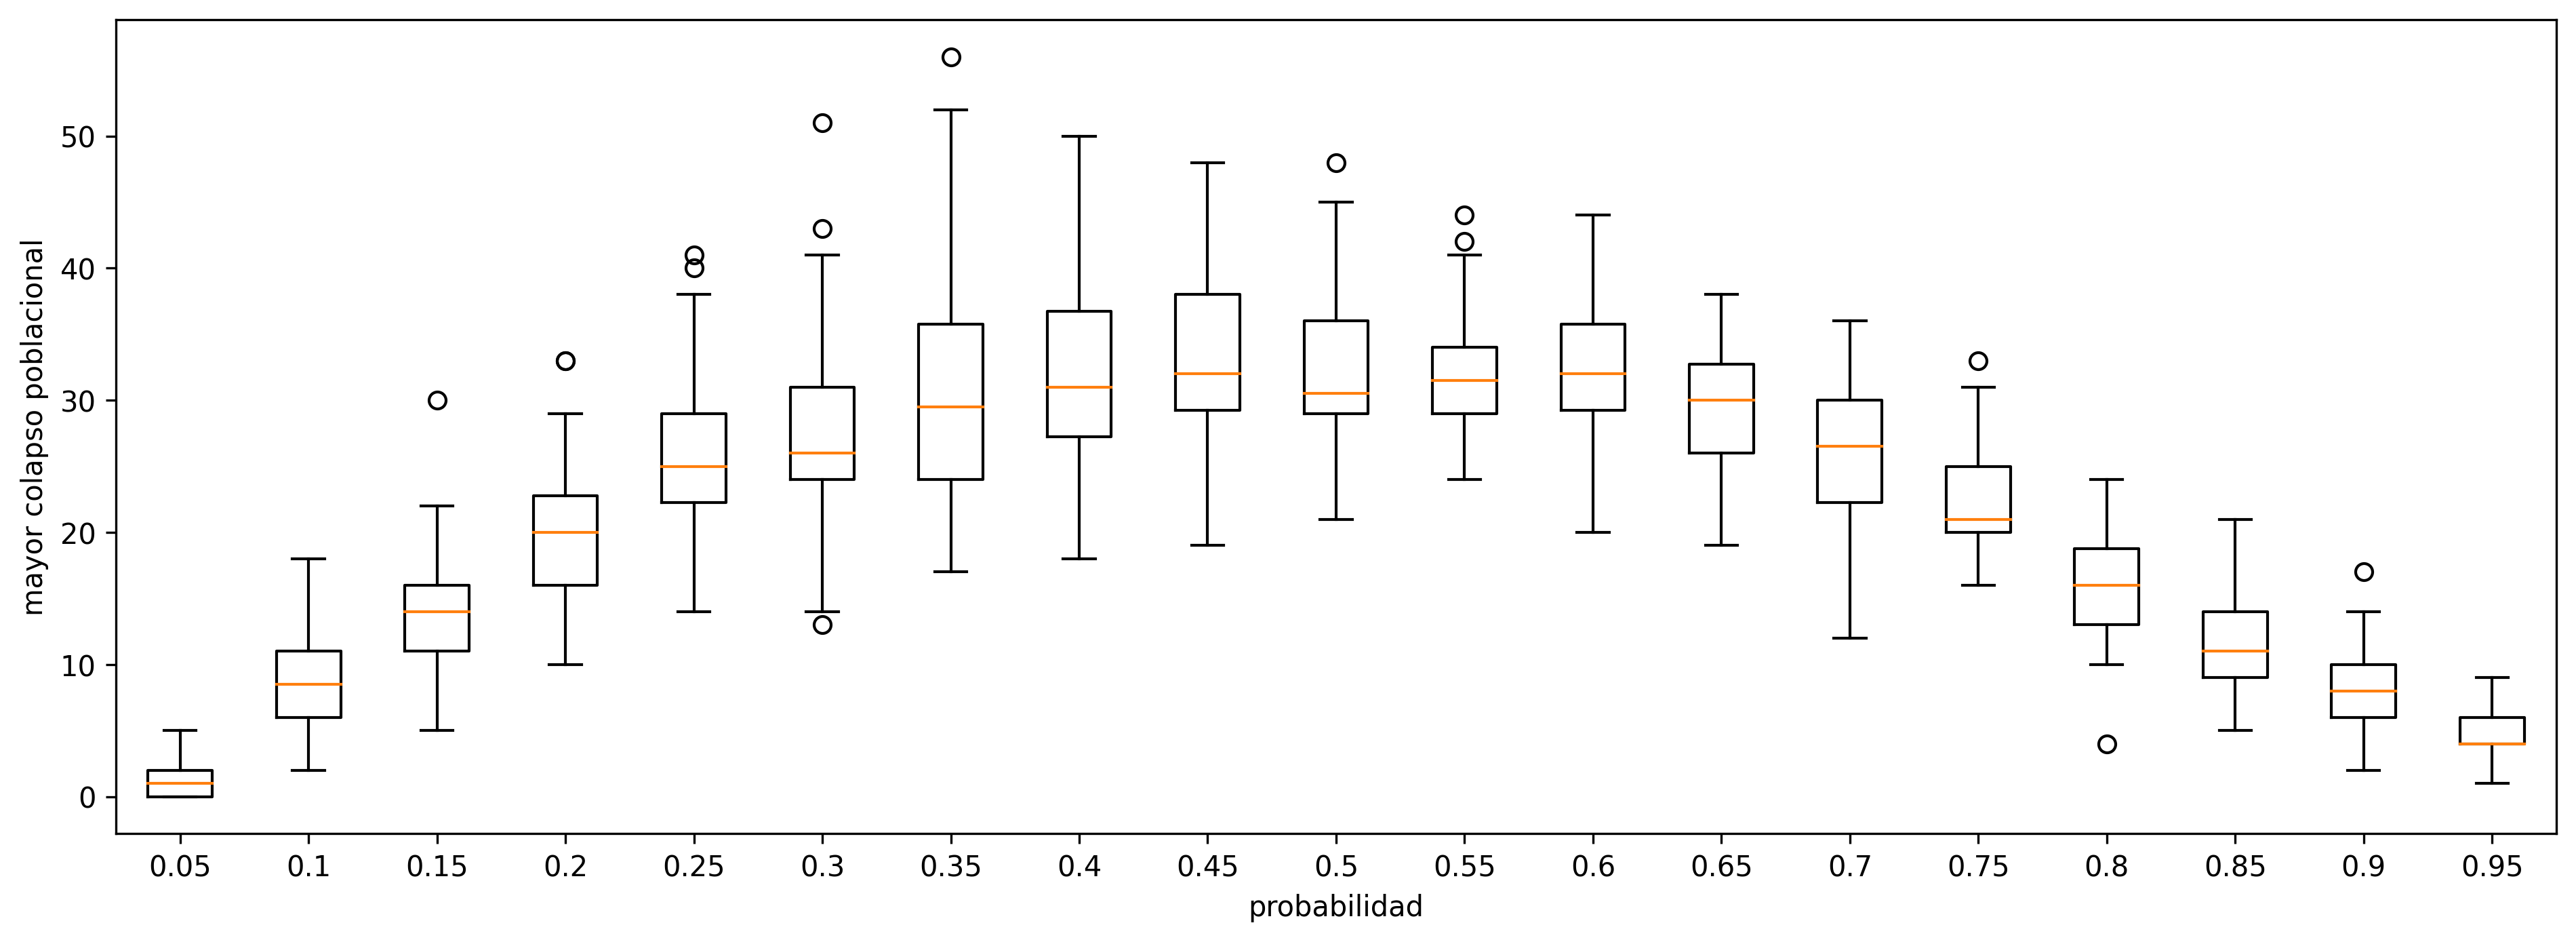
\includegraphics[width=\linewidth]{plot.png}
 \caption{Gráficas de caja de cada probabilidad}
 \label{colapso}
\end{figure}

\subsection{El mayor tiempo continuo de vida en una celda}
En este experimento, nos interesa encontrar cuantas iteraciones (de forma seguida) vive una celda, para ello se utiliza la función \texttt{vida\_maxima} \ref{lst:bar}. Dado que el juego de la vida cuenta con nueve iteraciones, una celda puede vivir a lo más nueve etapas. En cada corrida, para cada iteración, se guarda el estado de la celda en un vector para después calcular la vida máxima de dicha celda. Se utiliza el máximo de éstas para determinar la mayor vivencia de las celdas.

\begin{lstlisting}[label=lst:bar,caption=Función de vida máxima., frame = single, framexleftmargin=15pt]
def vida_maxima(a):
    n=0
    maxvida=[]
    for i in range (len(a)):
        n=n+a[i]
        if (a[i]==0):
            maxvida.append(n)
            n=0
        maxvida.append(n)
    return(max(maxvida))
\end{lstlisting} 
Los datos se recopilaron en un \texttt{data frame}, un fragmento de este se encuentra en el cuadro \ref{vmdatos} y
en la figura \ref{vida} se tiene los gráficos de caja para cada una de las probabilidades. En dicha figura se muestra la vida máxima que alcanza alguna celda de la malla. 

 En las probabilidades de 0.10, 0.75, 0.80, 0.85, 0.90 y 0.95, en promedio la vida máxima es de 2 iteraciones. En las probabilidades de 0.25 a 0.50 el promedio se mantiene constante en 5 iteraciones.
 
 \begin{table}
\centering
\caption{Fragmento de los datos recopilados}
\begin{tabular}{rrrrrrrr}
\hline 
Probabilidad & 1 & 2 & 3 & ... & 48 & 49 & 50 \\ 
\hline 
0.05 & 1 & 1 & 2 & ... & 1 & 1 & 1 \\ 
0.10 & 2 & 2 & 1 & ... & 3 & 1 & 1 \\ 
$\vdots$ & $\vdots$ & $\vdots$ & $\vdots$ & $\vdots$ & $\vdots$ & $\vdots$ & $\vdots$ \\ 
0.90 & 2 & 2 & 2 & ... & 2 & 2 & 2 \\ 
 0.95 & 2 & 2 & 2 & ... & 2 & 2 & 2 \\  
\hline
\end{tabular} 
\label{vmdatos}
\end{table}

\begin{figure}
\centering
 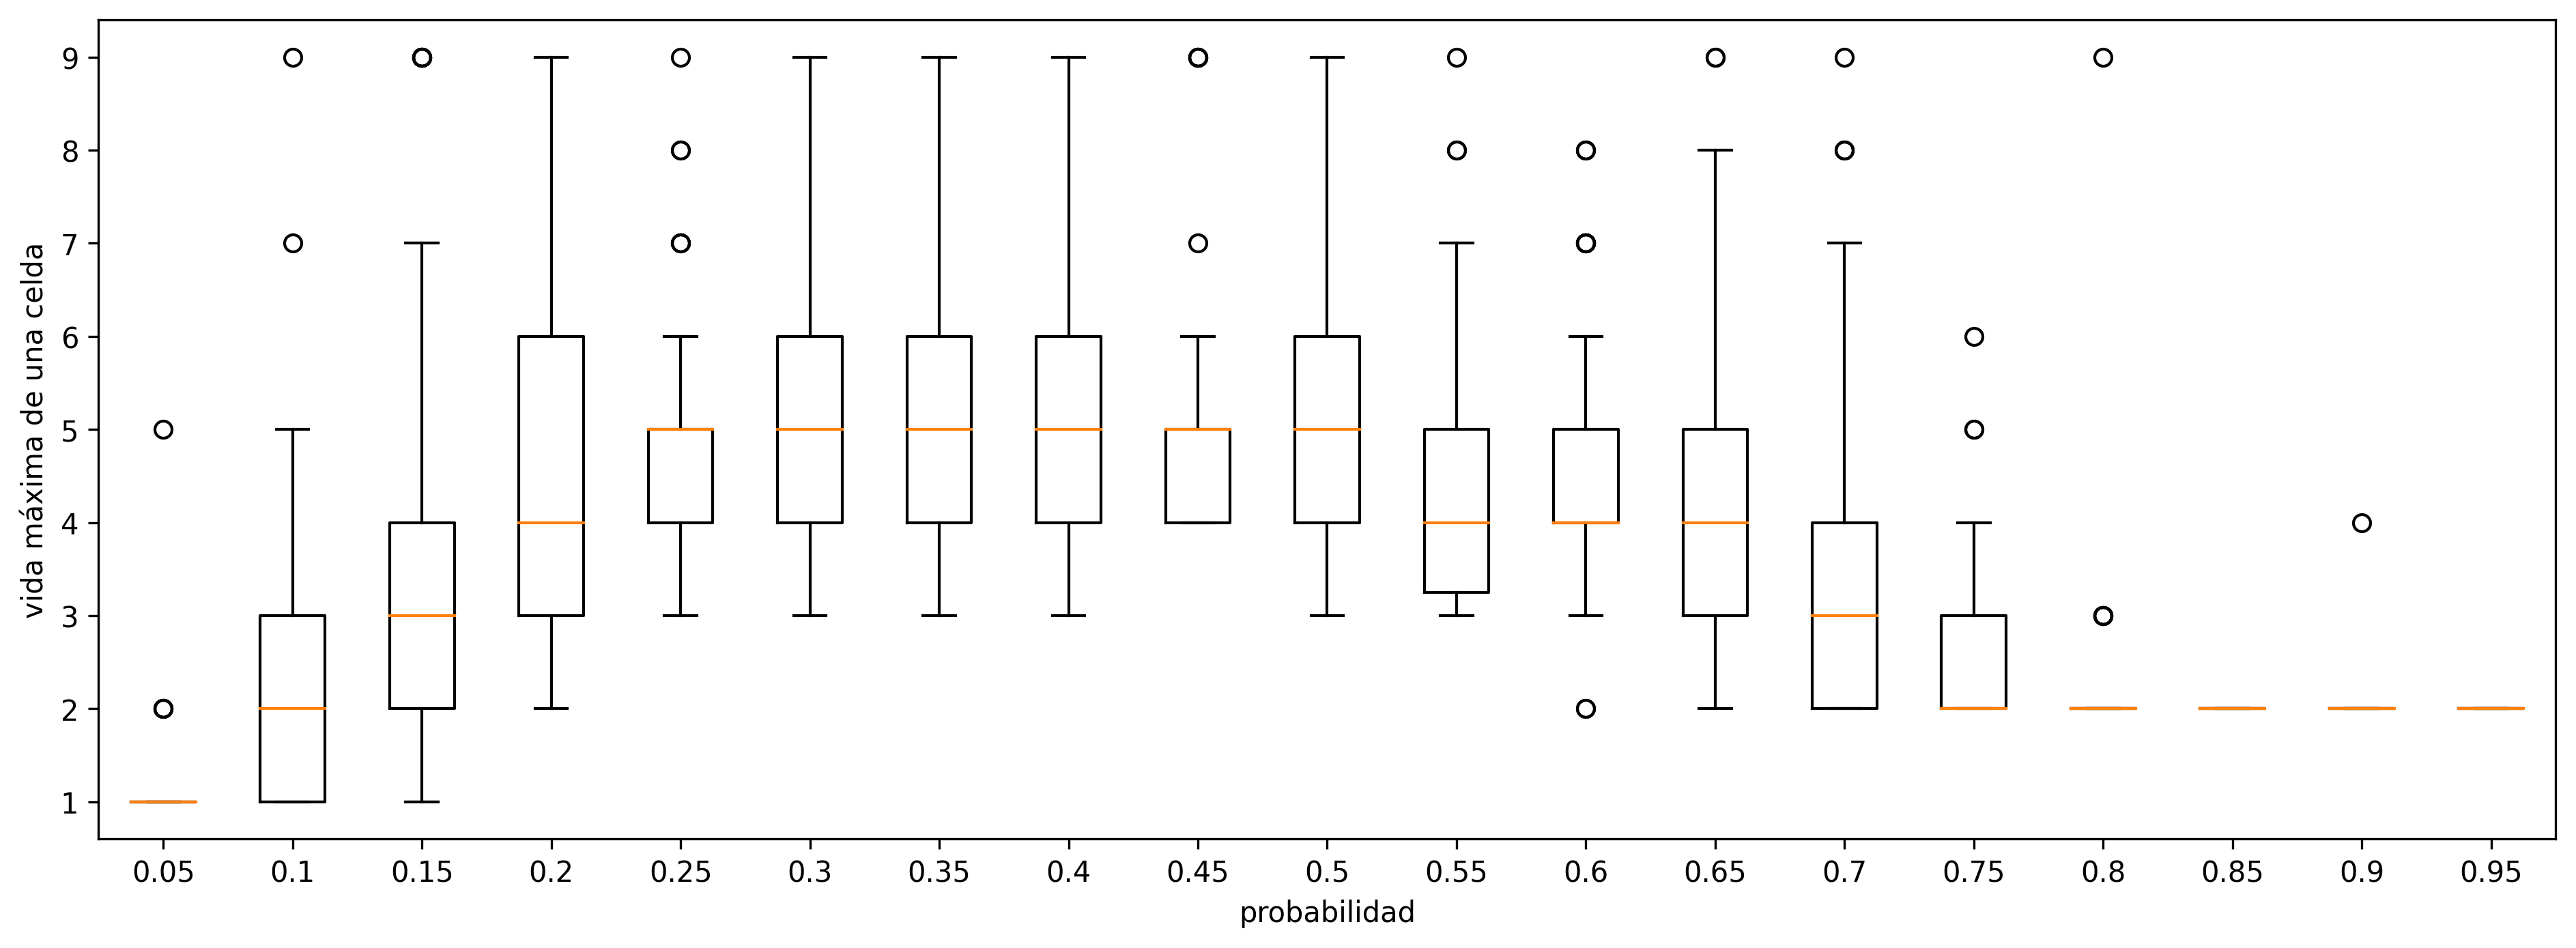
\includegraphics[width=\linewidth]{plot1.png}
 \caption{Gráficas de caja de cada probabilidad}
 \label{vida}
\end{figure}


\bibliographystyle{plain} 

\bibliography{Referencias}




\end{document}